\section{Wervelmassa als traagheid uit circulatie}

De massa van een knoopwervel in het Vortex Æther Model ontstaat niet als een fundamentele eigenschap, maar als gevolg van circulatie en weerstand tegen vervorming van de æther:

\subsection*{Circulatie als basis voor inertie}
De circulatie van een gesloten wervelpad wordt gegeven door:
\[
    \Gamma = \oint_{\partial S} \vec{v} \cdot d\vec{\ell} = 2\pi r_c C_e
\]
Deze grootheid is behouden in ideale fluïda (Helmholtz-theorema) en vormt een constante parameter voor elke knoopconfiguratie.

De implicatie hiervan is dat bij een gegeven $\Gamma$, elke verandering van $r_c$ (straal van de wervelkern) een overeenkomstige verandering in swirl $C_e$ vereist:
\[
    C_e = \frac{\Gamma}{2\pi r_c}
\]

\begin{figure}[h!]
    \centering
    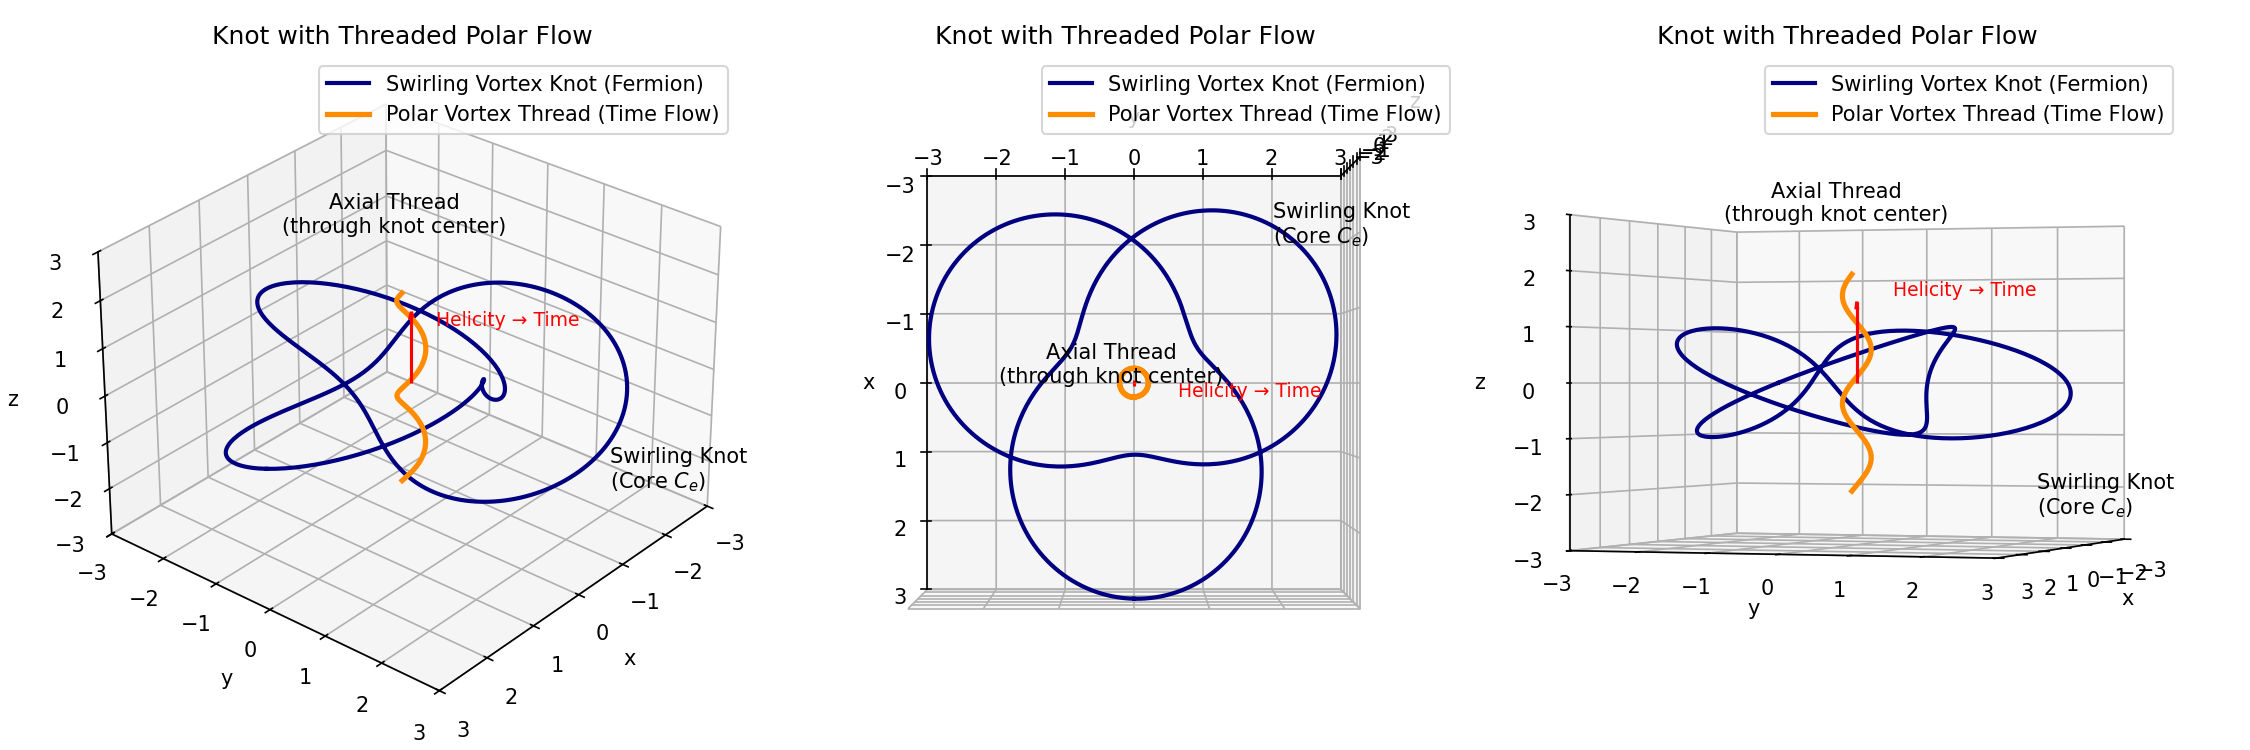
\includegraphics[width=0.98\textwidth]{KnotThreadedPolarFlow.png}
    \caption{Wervelknoop gekoppeld aan polaire draad: tijdsverloop als heliciteitstransport.}
\end{figure}
Deze relatie toont aan dat de swirl-snelheid $C_e$ een functie is van de circulatie $\Gamma$ en de kernstraal $r_c$. Dit betekent dat massa in VAM niet een intrinsieke eigenschap is, maar voortkomt uit de geometrie van de knoop en de dynamica van de wervelstructuur.

\subsection*{Afleiding van effectieve massa}
Kinetische energie gekoppeld aan deze swirl is:
\[
    E = \frac{1}{2} \rho_\text{\ae} C_e^2 V = \frac{1}{2} \rho_\text{\ae} \left( \frac{\Gamma}{2\pi r_c} \right)^2 \cdot \frac{4}{3}\pi r_c^3
\]
\[
    \Rightarrow E = \frac{\rho_\text{\ae} \Gamma^2}{6\pi r_c}
\]

Deze energie kunnen we associëren met de klassieke inertieformule $E = \frac{1}{2} m C_e^2$, waaruit een effectieve massa volgt:
\[
    m_\text{eff} = \frac{\rho_\text{\ae} \Gamma^2}{3\pi r_c C_e^2}
\]

Dit toont dat massa direct voortkomt uit:
- De circulatiekracht $\Gamma$
- De geometrie van de knoop ($r_c$)
- De wervelsnelheid $C_e$

\subsection*{Vergelijking met klassieke inertie}
Ter vergelijking:
\[
    m \sim \frac{\text{traagheidsenergie}}{C_e^2} \quad \text{vs.} \quad E = m c^2 \text{ in SR}
\]
In VAM is $C_e$ de lokale swirl-constante, en $c$ de propagatiesnelheid van verstoringen. Dat betekent dat massa in VAM \textbf{afleidbaar is uit
geometrie en behoud} — en niet fundamenteel postulaat.

\subsection*{Fermion-massaterm in Lagrangian}
Met bovenstaande afleiding kunnen we de massaterm van een fermion schrijven als:
\[
    \mathcal{L}_\text{massa} = m_f C_e r_c \cdot \bar{\psi}_f \psi_f
\]
waarbij $m_f$ hier proportioneel is aan $\rho_\text{\ae}$ en $\Gamma^2$ van de knoopwervel. Dit vervangt de standaard Yukawa-koppeling door een fluïdumeigenschap.